\documentclass[handout]{beamer}

\usetheme[progressbar=frametitle]{metropolis}
\usepackage{appendixnumberbeamer}
\usepackage{booktabs}
\usepackage{amsmath}
\usepackage{amssymb}
\usepackage{tcolorbox}
\definecolor{metropolisblue}{RGB}{39, 59, 94}
\usepackage{xcolor}

% Define custom colors
\definecolor{myblue}{HTML}{007AFF}
\definecolor{mygreen}{HTML}{4CD964}
\definecolor{myred}{HTML}{FF3B30}
\definecolor{myorange}{HTML}{FF9500}



% Begin document
    % \begin{frame}{One Equation Throughout the Course}
    %    Let's consider an example to understand the concept of maximum likelihood estimation and maximum aposteriori estimate. Lets' consider the Electricity consumption vs. Occupancy data.
        
    % \end{frame}



\begin{document}

% \begin{frame}{Univariate Normal Distribution}
%     The probability density function of a univariate normal distribution is given by:
    
%     \begin{equation}
%     f(x|\mu, \sigma^2) = \frac{1}{\sqrt{2\pi\sigma^2}}\exp\left(-\frac{(x-\mu)^2}{2\sigma^2}\right)
%     \end{equation}
    
%     Let us assume we have a dataset $D = \{x_1, x_2, \ldots, x_n\}$, where each $x_i$ is an independent sample from the above distribution. 
%     We want to estimate the parameters $\theta = \{\mu, \sigma\}$ from the data.
    
%     Our likelihood function is given by:
%     \begin{equation}
%     P(D|\theta) = \mathcal{L}(\mu, \sigma^2) = \prod_{i=1}^n f(x_i|\mu, \sigma^2)
%     \end{equation}
    
    
%     \end{frame}

    \begin{frame}{One Equation Throughout the Course}
        \begin{itemize}
            \item Consider the following dataset:
        \end{itemize}
    \begin{figure}
        \centering
        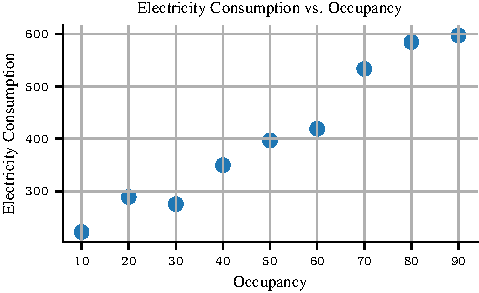
\includegraphics[width=0.8\textwidth]{../figures/introduction-madhav/data.pdf}
    \end{figure}
    \begin{itemize}
        \item What could be a good fit for this dataset?
        \item Does this follow the general trend?
    \end{itemize}
    \end{frame}


    \begin{frame}{One Equation Throughout the Course}
        \begin{itemize}
            \item Some possible fits:
        \end{itemize}
        \begin{figure}
            \centering
            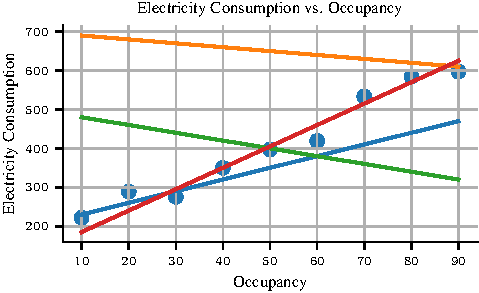
\includegraphics[width=0.8\textwidth]{../figures/introduction-madhav/manyfit.pdf}
        \end{figure}
        
    \end{frame}

    \begin{frame}{One Equation Throughout the Course}
        \begin{figure}
            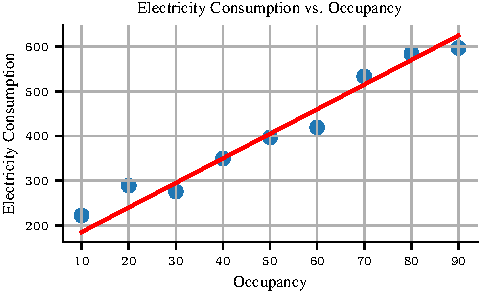
\includegraphics{../figures/introduction-madhav/bestfit.pdf}
        \end{figure}
        
    \end{frame}

    \begin{frame}{One Equation Throughout the Course}
        \begin{itemize}
            \item Why do we need Bayes theorem if we can get the best fit using conventional methods?
            \item Let's consider the case of two hostels and their electricity consumptions.
        \end{itemize}
        
    \end{frame}

    \begin{frame}{One Equation Throughout the Course}
        \begin{itemize}
            \item Hostel A's electricity consumption:
        \end{itemize}
        \begin{figure}
            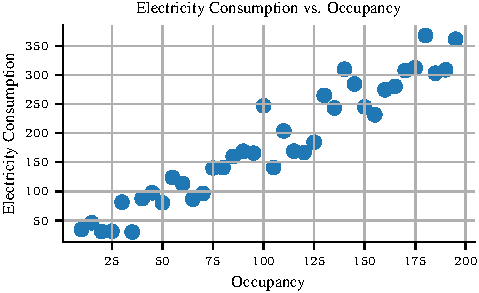
\includegraphics{../figures/introduction-madhav/mle_good.pdf}
        \end{figure}
        \begin{itemize}
            \item Does this follow the general trend?
        \end{itemize}
    \end{frame}


    \begin{frame}{One Equation Throughout the Course}
        \begin{figure}
            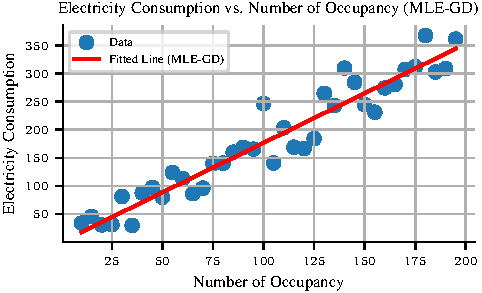
\includegraphics{../figures/introduction-madhav/mle_good_fit.pdf}
        \end{figure}
        
    \end{frame}

    \begin{frame}{One Equation Throughout the Course}
        \begin{itemize}
            \item Hostel B's electricity consumption:
        \end{itemize}
        \begin{figure}
            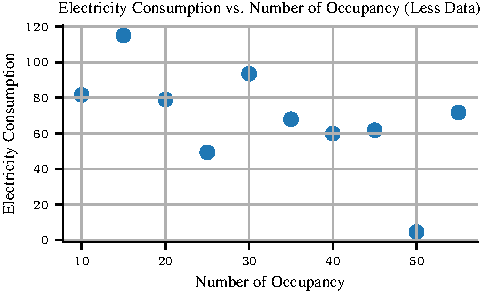
\includegraphics{../figures/introduction-madhav/mle_bad.pdf}
        \end{figure}
        \begin{itemize}
            \item Does this follow the general trend?
        \end{itemize}
    \end{frame}

    \begin{frame}{One Equation Throughout the Course}
        \begin{figure}
            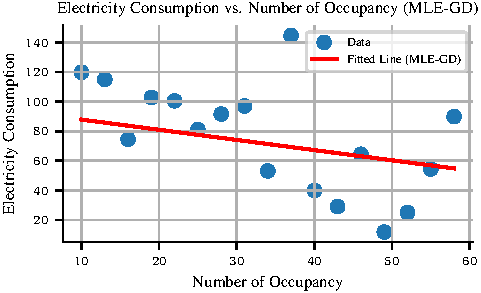
\includegraphics{../figures/introduction-madhav/mle_bad_fit.pdf}
        \end{figure}
        
    \end{frame}

    % \begin{frame}{One Equation Throughout the Course}
    %     \begin{figure}
    %         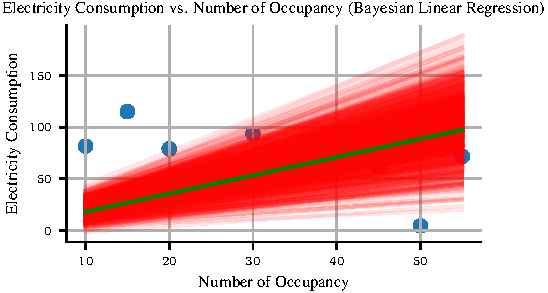
\includegraphics{../figures/introduction-madhav/mle-knowledge.pdf}
    %     \end{figure}
        
    % \end{frame}

\end{document}